\section{Approach}

\subsection{Problem}
We want to predict the location of an user's phone based on the sensor data collected on the phone. 
From our observations, the most common states of the phone would be in a user's: backpack, pocket, hand, and on a table. 

\subsection{Features}
For creating features, the relevant sensor data were the Accelerometer readings (X, Y, Z values), Number of unlocks, Number of screen touches, and Number of times the screen turned on/off. For each window of 0.5s of these raw sensor readings, we generated the following features:

\begin{enumerate}
\item \textit{Total number of phone unlocks}
\item \textit{Total number of phone touches}
\item \textit{Fraction of window that phone screen was on}
\item \textit{Mean acceleration each in X, Y, Z directions}
\item \textit{Std. deviation of acceleration each in X, Y, Z directions}
\item \textit{Mean magnitude of acceleration each in X, Y, Z directions}
\item \textit{Std. deviation of magnitude of acceleration each in X, Y, Z directions}
\item \textit{If phone is flat (handcrafted feature explained below)}
\end{enumerate}

The "If phone is flat" feature was a boolean feature derived from the raw accelerometer readings. 
The feature was 1 if the equation below held true, and 0 otherwise.
$$ (Mean X Accel. Magnitude) < 1.0 and (Mean Y Accel. Magnitude ) < 1.0 and |9.8 - (Mean Z Accel. Magnitude)| < 1.0 $$

\subsection{Architecture}
Our architecture consisted of two distinct sections: a convolutional section and a dense, fully connected section. 
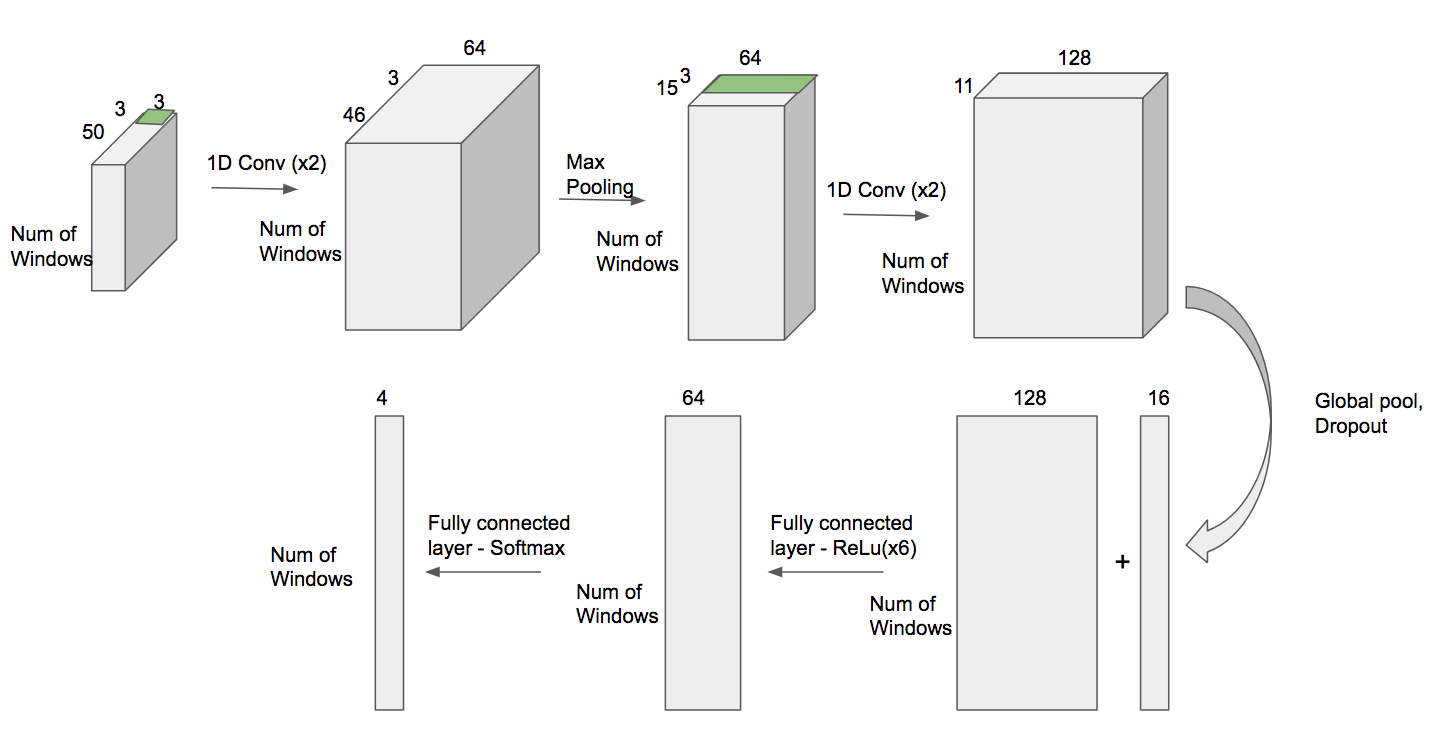
\includegraphics{convnet}

Specifically in the convolution section, we use the raw acceleration data, which includes the acceleration in the x, y, z direction. 
After multiple 1 dimensional convolution layers, max and global pooling, and dropout layers, we concantenate the 16 features from the section above in order to incorporate the other features. 
We chose to separate out the acceleration and the other features in order to take advantage of the potentially "periodic" behavior of a user's acceleration in certain positions (e.g. walking).

After the concatenation of inputs, our model has 6 dense layers with 4 outputs, which match the four classes listed previously. 